\documentclass[10pt,french]{article}
\input preambule_2013

\newcounter{exoc}
\newenvironment{exoc}[1]{%
  \refstepcounter{exoc}\textbf{Exercice \theexoc} :\hfill {\textbf{(#1)}}\par
  \medskip}%
{\medskip}

\begin{document}


\pieddepage{}{}{}

\begin{center}
\begin{tabularx}{\textwidth}{|>\centering m{2.5cm}|>\centering X|>{\centering\arraybackslash} m{2.5cm}|}
	\hline
		1\iere \bsc{s.t.m.g.} &  Mercredi 18 décembre \np{2013} & \textbf{Statistiques} \\
	\hline
		\multicolumn{3}{|c|}{\bsc{Contrôle de mathématiques}} \\
	\hline
        \multicolumn{1}{|r}{\bsc{Nom}:} & \multicolumn{2}{l|}{} \\
		\multicolumn{1}{|r}{Prénom:} & \multicolumn{2}{l|}{} \\
	\hline
        \multicolumn{3}{|l|}{\bfseries Note et observations :} \\[1cm]
    \hline
\end{tabularx}\bigskip

{\itshape
La qualité et la précision de la rédaction seront prises en compte dans l'appréciation des copies.\par
Le barème est indicatif.
}
\end{center}

\begin{exoc}{1 + 1 + 1 + 3 = 6 pts}
    Un bureau a fait une étude statistiques auprès de ses employés pour connaître leur temps de trajet quotidien en minutes pour se rendre à leur travail.
    \begin{center}
        \begin{tabular}{|>\bfseries c|*{8}{>{\centering\arraybackslash}m{1.25cm}|}}
            \hline
                Temps du trajet & $\intervallefo{0}{10}$ & $\intervallefo{10}{20}$ & $\intervallefo{20}{30}$ & $\intervallefo{30}{40}$ & $\intervallefo{40}{50}$ & $\intervallefo{50}{60}$ & $\intervallefo{60}{70}$ & $\intervallefo{70}{80}$ \\
            \hline
                Effectifs & 6 & 16 & 24 & 10 & 13 & 15 & 4 & 2 \\
            \hline
                Centre de classe & &&&&&&& \\
            \hline
        \end{tabular}
    \end{center}
    
    \begin{enumerate}
        \item Compléter le tableau.
        \item Quel est le pourcentage de personnes pour lesquelles le temps de trajet est strictement inférieur à $1$ heure ? Arrondir au dixième près.
        \item En utilisant les centres de classes, calculer le temps moyen $\overline m$ par personne. Arrondir au dixième près.
        \item En utilisant les centres de classes, calculer et \textbf{interpréter} la médiane $M_e$, le premier quartile $Q_1$ et le troisième quartile $Q_3$.
    \end{enumerate}
\end{exoc}

\begin{exoc}{1 + 1 + 1 + 1 + 3 = 7 pts}
    Une machine est programmée pour fabriquer une pièce dont le diamètre doit être de $5~mm$. Pour cela, l'opérateur règle la machine sur cette valeur. On observe toutefois des variations dans les diamètres des pièces fabriquées, ceci est inévitable mais il faut toutefois rester dans des limites acceptables.\par
    Le service Qualité de l'entreprise prélève un échantillon de $40$ pièces en vue de contrôler la machine. Les résultats sont dans le tableau suivant :

    \begin{center}
        \begin{tabular}{|>{\bfseries\centering} m{3cm}|*{10}{>{\centering\arraybackslash}m{0.75cm}|}}
            \hline
                Diamètre des pièces (en $mm$)& $4,5$ & $4,6$ & $4,7$ & $4,8$ & $4,9$ & $5$ & $5,1$ & $5,2$ & $5,3$ & $5,4$ \\
            \hline
                Effectifs & $1$ & $1$ & $4$ & $9$ & $10$ & $5$ & $4$ & $2$ & $3$ & $1$ \\
            \hline
        \end{tabular}
    \end{center}

    \begin{enumerate}
        \item En utilisant la fonction \texttt{stats} de la calculatrice, déterminer la valeur \textbf{exacte} du diamètre moyen des pièces.\par On le notera $\overline d$.
        \item En utilisant la fonction \texttt{stats} de la calculatrice, déterminer l'écart-type de cette série.\par Arrondir le résultat au \textbf{millième près}. On le notera $\sigma$.
        \item En détaillant les calculs effectués, déterminer les intervalles $I_1 = \intervalleff{\overline d - \sigma}{\overline d + \sigma}$ et $I_2 = \intervalleff{\overline d - 2\sigma}{\overline d + 2\sigma}$.
        \item La production de la machine est jugée satisfaisante si environ $66\%$ des pièces appartiennent à l'intervalle $I_1$ et $95\%$ des pièces appartiennent à l'intervalle $I_2$.\par
        La production de la machine est-elle correcte ? Justifier précisément.
    \end{enumerate}
\end{exoc}

\vfill

\begin{center}
    \textbf{Tourner la page pour l'exercice 3 !}
\end{center}

\vfill\clearpage

\textbf{L'exercice 3 est à faire entièrement sur le sujet.}\medskip

\begin{exoc}{1 + 1,5 + 1 + 1,5 + 2 = 7 points}
    La série statistique ci-dessous représente la répartition des filles d'un club de sport en fonction de leur âge.

    \begin{center}
        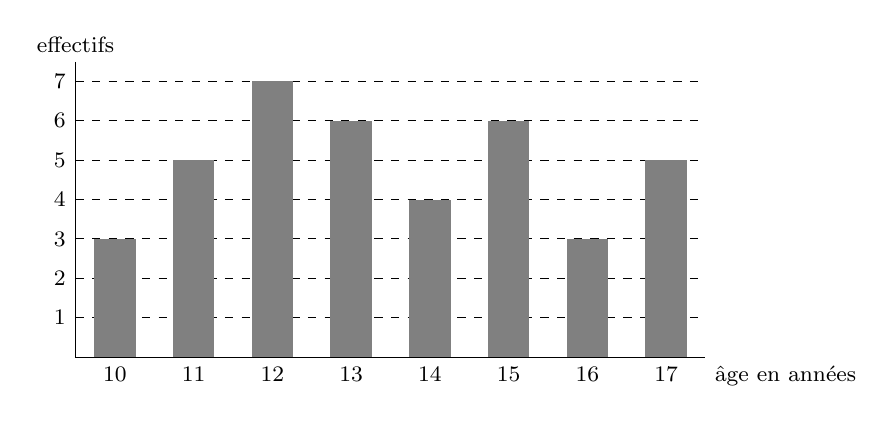
\begin{tikzpicture}[yscale=0.5]
            \foreach \x in {1,...,7} \draw[dashed] (0,\x) -- (8,\x);
            \foreach \x in {1,...,7} \draw (0,\x) node[left] {\footnotesize $\x$};
            \draw[line width = 0.2pt] (0,7.5) node[above] {\footnotesize effectifs} -- (0,0) -- (8,0) node[below right] {\footnotesize âge en années};
            \draw[line width = 15pt,color=gray] (0.5,0) -- (0.5,3);
            \draw[line width = 15pt,color=gray] (1.5,0) -- (1.5,5);
            \draw[line width = 15pt,color=gray] (2.5,0) -- (2.5,7);
            \draw[line width = 15pt,color=gray] (3.5,0) -- (3.5,6);
            \draw[line width = 15pt,color=gray] (4.5,0) -- (4.5,4);
            \draw[line width = 15pt,color=gray] (5.5,0) -- (5.5,6);
            \draw[line width = 15pt,color=gray] (6.5,0) -- (6.5,3);
            \draw[line width = 15pt,color=gray] (7.5,0) -- (7.5,5);
            \foreach \x in {10,...,17} \draw (\x-9.5,0) node[below] {\footnotesize $\x$};
        \end{tikzpicture}
    \end{center}

    \begin{enumerate}
        \item Combien y a t-il de filles entre $10$ et $17$ ans dans ce club ? Justifier en écrivant le calcul effectué.\par\tikz{\draw (0,0) rectangle (\linewidth-10pt,2);}
        \item En utilisant la fonction \texttt{stats} de la calculatrice, compléter les phrases suivantes :\medskip
        \begin{enumerate}
            \item $25\%$ des filles ont un âge inférieur ou égal à \ldots \bigskip
            \item $75\%$ des filles ont un âge inférieur ou égal à \ldots \bigskip
            \item $50\%$ des filles ont un âge inférieur ou égal à \ldots
        \end{enumerate}
        \item Donner l'intervalle interquartile et interpréter le résultat à l'aide d'un pourcentage.\par\tikz{\draw (0,0) rectangle (\linewidth-10pt,2);}
        \item Le diagramme en boîte ci-dessous représente la répartition des garçons en fonction de leur âge dans le même club de sport.\par
        Représenter ci-dessous le digramme en boîte représentant la répartition des filles.
            
            \begin{center}
    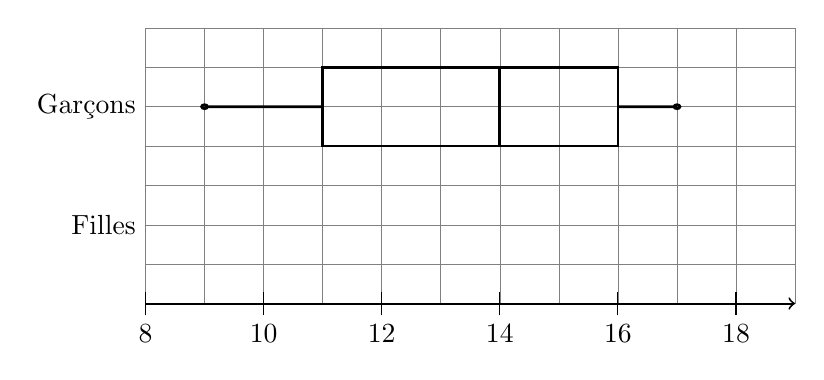
\begin{tikzpicture}[xscale=1.5]
        \draw[help lines] (0,0) grid[step=5mm] (5.5,3.5);
        \draw[->,line width=0.7pt] (0,0) -- (5.5,0);
        \foreach \x in {8,10,...,18} \draw (\x/2-4,-0.15)node[below] {\x} -- (\x/2-4,0.15);
% diagramme en boîte 1 :
        \def\y{2.5}
        \def\mini{9}\def\maxi{17}
        \def\qA{11}\def\med{14}\def\qB{16}
        \draw[line width=1pt] (\mini/2-4,\y) circle (0.7pt)--(\mini/2-4,\y) -- (\qA/2-4,\y);
        \draw[line width=1pt] (\qA/2-4,\y-0.5) rectangle (\qB/2-4,\y+0.5);
        \draw[line width=1pt] (\qB/2-4,\y) -- (\maxi/2-4,\y)--(\maxi/2-4,\y) circle (0.7pt);
        \draw[line width=1pt] (\med/2-4,\y-0.5)--(\med/2-4,\y+0.5);
        \draw (0,\y) node[left] {Garçons};
% diagramme en boîte 2 :
        \def\y{1}
        \def\mini{10}\def\maxi{17}
        \def\qA{12}\def\med{13}\def\qB{15}
%        \draw[line width=1pt] (\mini/2-4,\y) circle (0.7pt)--(\mini/2-4,\y) -- (\qA/2-4,\y);
%        \draw[line width=1pt] (\qA/2-4,\y-0.25) rectangle (\qB/2-4,\y+0.25);
%        \draw[line width=1pt] (\qB/2-4,\y) -- (\maxi/2-4,\y)--(\maxi/2-4,\y) circle (0.7pt);
%        \draw[line width=1pt] (\med/2-4,\y-0.25)--(\med/2-4,\y+0.25);
        \draw (0,\y) node[left] {Filles};
    \end{tikzpicture}
\end{center}
    \item Entre les garçons et les filles, quels sont ceux dont les âges sont les plus dispersés ? Donner deux explications précises à la réponse.\par\tikz{\draw (0,0) rectangle (\linewidth-10pt,3.75);}
    \end{enumerate}
\end{exoc}

\end{document} 